\subsection{Measurement of Jet Resolution Tails}
\label{sec:res_tails}

One of the most promising signatures of physics beyond the standard model involves events with multiple jets and a large missing transverse energy \met. A background to this signal is expected from QCD multijet production where \met can originate, e.g. from fluctuations in the detector response to jets. One way to estimate the QCD background in the high \met signal region is to smear particle-level multijet events with parameterizations of the full jet \pt resolution functions that model both the Gaussian core and the tails of the distributions. It is therefore important to quantify the non-Gaussian 
component of the jet \pt resolution in order to predict accurately the QCD background.

Two complementary studies of resolution tails are presented, using dijet and 
$\gamma+$jet  events. For these studies, the focus is on the PF jet 
reconstruction, since it provides the best jet \pt resolution and is adopted in the primary physics analyses most sensitive to the impact of the jet \pt resolution tails.

\subsubsection{Dijet Asymmetry Measurement}

The full resolution functions can be derived using the generator-level MC 
information in 
the simulation. To validate the MC simulation description of the 
\pt-resolution  tails with the currently available data samples, the 
fractional number of events in the tail regions of the dijet \pt asymmetry 
distributions is compared between data and simulation.

As shown before (Table ~\ref{tab:ResFit:ScalingFactors}), the 
central-core widths of the response and asymmetry 
distributions differ between data and MC samples. The adopted strategy is 
to  adjust the MC response distributions to have the same core resolutions 
in MC simulations as in data. Then, the fraction of events in a given 
asymmetry  window in the tail of the distribution is calculated with both 
data and MC samples. Different tail regions have been studied; here the 
results 
for the window \mbox{$2.5\sigma - \infty$} are presented. These fractions 
are observed to depend on the threshold on the third-jet \pt, and are 
therefore extrapolated to zero.
The measured ratio between data and MC fractions from asymmetry is used to 
correct the fraction from generator-level MC  in the form of a scaling 
factor. Since the  dijet asymmetry distribution is symmetric by 
construction, the measured tail-scaling factors average over the low and 
the 
high response tails. To validate the method and to quantify biases caused 
by the event selection, the extrapolated fractions in the MC simulation have 
been compared to the expectation from the asymmetry  
from the generator-level response. Small deviations in the MC closure 
are taken  as a source of systematic uncertainty. Other systematic 
uncertainties have been estimated from the extrapolation procedure and 
from the scaling of the central-core widths between data and MC samples.
The final results for the scaling factors are presented in 
Fig.~\ref{fig:Asym:ScalingFactors}. These results demonstrate that, 
given the current data statistics, the observed data over MC ratios of 
the resolutions tails are within a factor of 1.5.

\begin{figure}[ht]
 \centering
  \begin{tabular}{cc}
    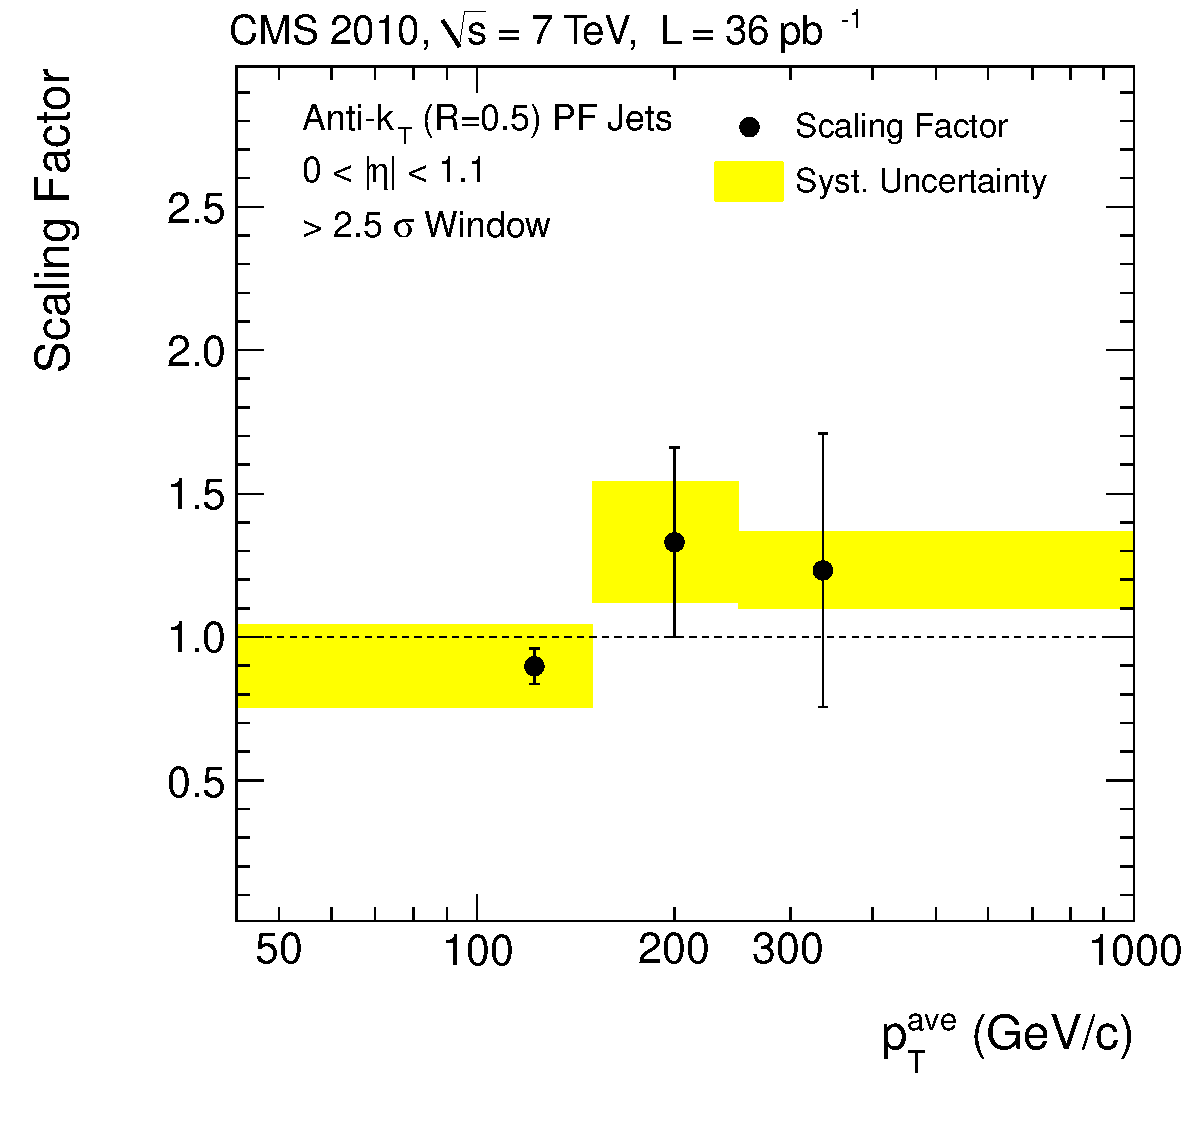
\includegraphics[width=0.45\textwidth]{Figures/JER/figs/res_tails/TailScalingFactorsSig25-Inf_PF_Eta0} &
    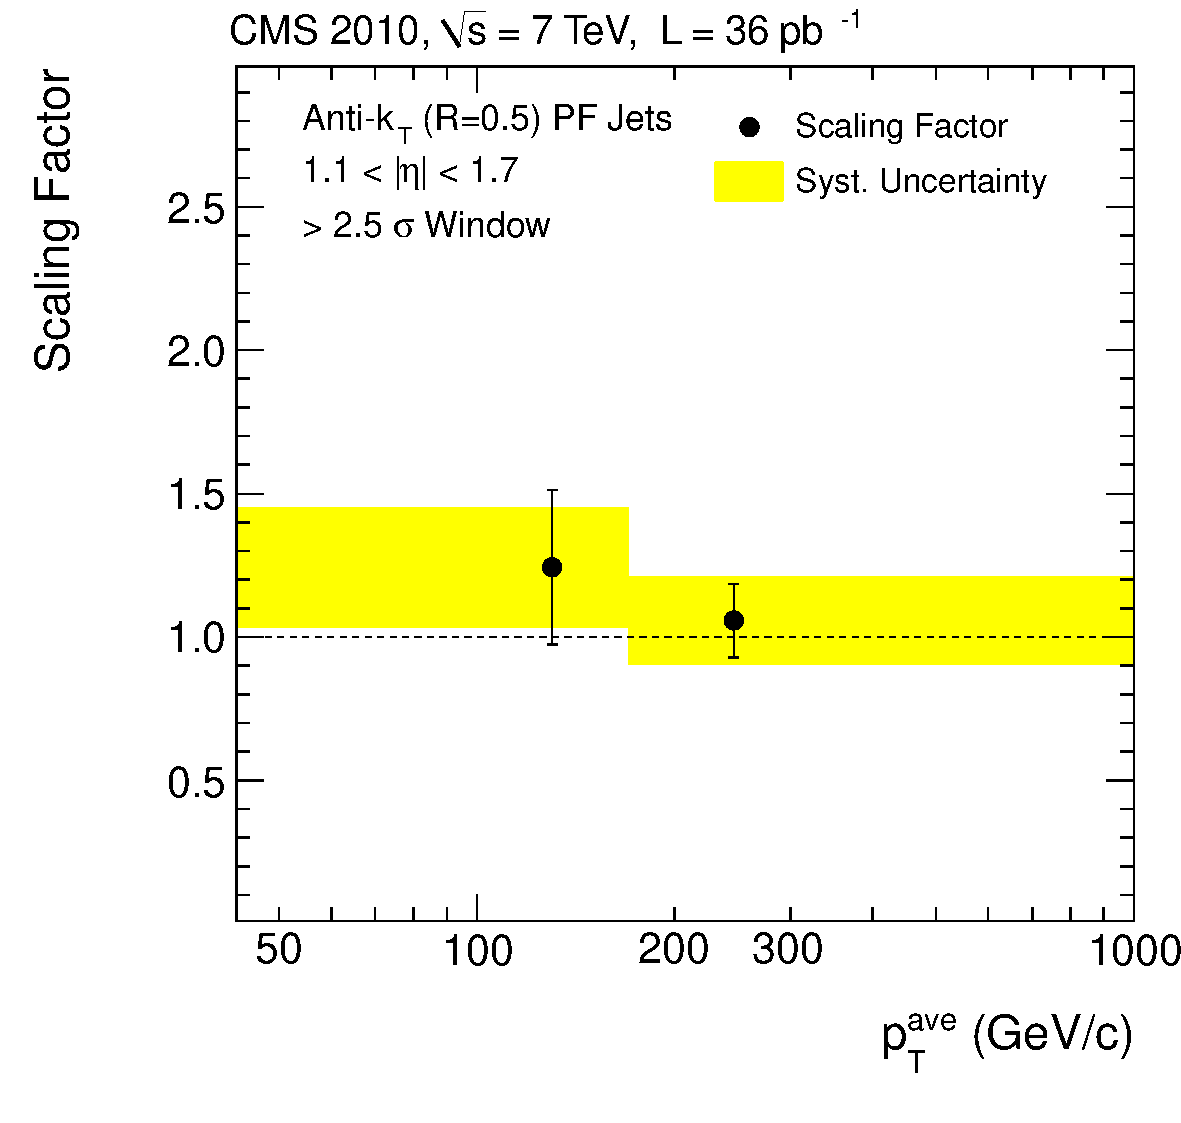
\includegraphics[width=0.45\textwidth]{Figures/JER/figs/res_tails/TailScalingFactorsSig25-Inf_PF_Eta1} \\
 \end{tabular}
  \caption{The data/MC scaling factors for the tails of the resolutions observed in the dijet 
samples for different $\eta$ and \pt bins, using the $>2.5\sigma$ window.}
  \label{fig:Asym:ScalingFactors}
\end{figure}


\subsubsection{$\gamma$ + Jet Measurement}

This method uses the \pt balance in $\gamma$+jet events to estimate the 
non-Gaussian tails of the resolution. It can be used separately for the 
low- and high-response tails because the response distribution 
is not symmetric  as in the case of dijet measurement. The number of 
events  outside 2.5$\sigma$ range is counted in bins of $\pt^{\gamma}$, to 
compare the resolution tails 
from the MC simulation to the level observed in data. An example 
distribution is shown 
in Fig.~\ref{fig:tailFits} (left) for the  $32<\pt^{\gamma}<52\GeV$ bin and central $\eta$, and the ratio of the number of tail events in data and MC
samples  vs. $\pt^{\gamma}$ is shown on the right, as function of 
$\pt^{\gamma}$. 
The available statistics in data do not allow to measure the resolution tails
with precision, but a constant fit  to the ratio is consistent within 
uncertainties with the study using the dijet sample, and thereby provides 
a cross-check.

\begin{figure}[htbp]
\begin{center}
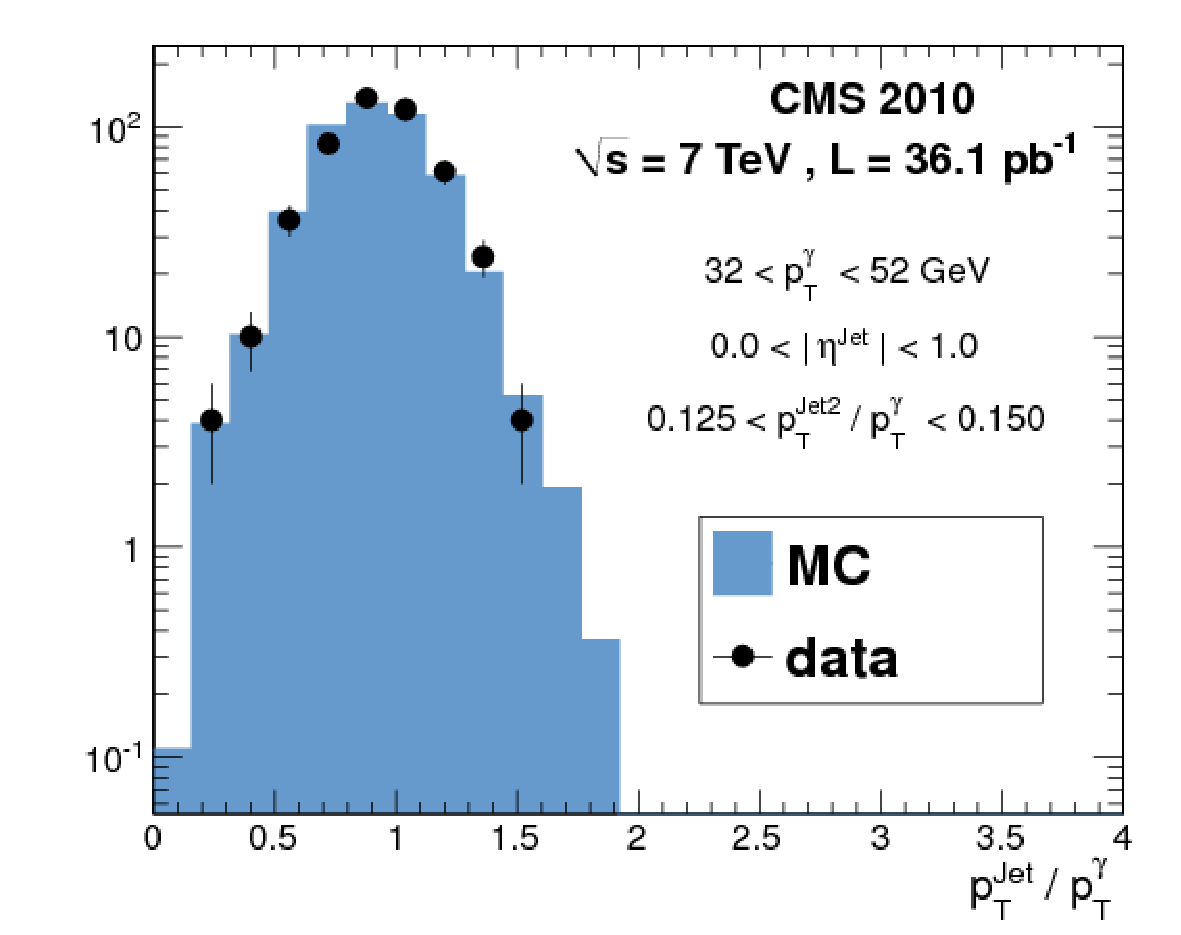
\includegraphics[width=0.45\textwidth]{Figures/JER/figs/res_tails/MC_data_32to52GeV_125to150.pdf}
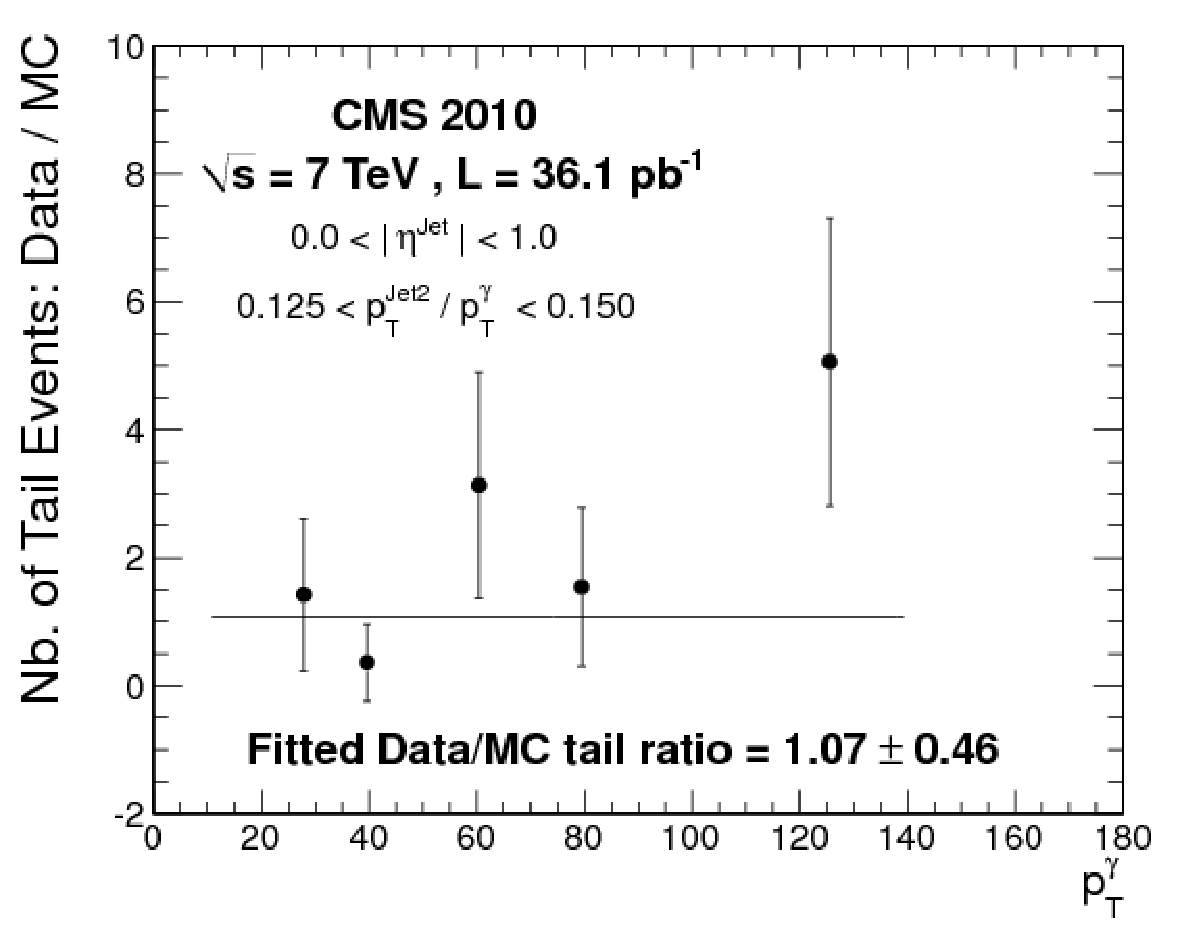
\includegraphics[width=0.45\textwidth]{Figures/JER/figs/res_tails/TailRatio_DataOverMC.pdf}
\end{center}
\caption[]{An example jet \pt resolution function for the $32<\pt^{\gamma}<52\GeV$ bin (left); ratio of the number of tail 
events  in data and MC samples vs. $\pt^\gamma$ (right).} 
\label{fig:tailFits}
\end{figure}



